%!TEX root = ../rapport.tex

\chapter{Graph Drawing}\label{chap:graph_drawing}

A \emph{graph drawing} is an embedding of the abstract, mathematical concept
of a graph on a two-dimensional surface. A \emph{graphic standard} is the
translation between the abstract graph and graphic symbols representing the
graph. Different graphic standards exist, but the most common ones represent
vertices by dots or filled circles and edges $(u,v)$ by curves connecting the
symbols representing $u$ and $v$. In this chapter we will briefly summarize
the different, relevant graphic standards and methods for drawing them.

Battista et al. give a more thorough overview of the literature in several
different areas of research related to graph drawing in \cite{DiBattista1994}.

\section{Aesthetics}

Graph drawing was motivated by the need for conveying information embedded in
graphs to humans, for instance in the fields of VLSI circuit design, social
network analysis and algorithm visualization. Thus, the quality of a graph
drawing depends heavily on its ability to clearly convey its information,
making it easy for the reader to decipher it. Different \emph{aesthetic
measures} have therefore been developed, depending on the type of information
that the graph must deliver. Common aesthetics are \cite{DiBattista1994}:
\begin{itemize}
	\item The distance between adjacent nodes is
	sought to be minimized, since it can be difficult to get an overview of the
	drawing if edges tend to be very long.
	
	\item The area covered by the graph -- the minimum bounding box of the 
	graph -- can also be an important factor, especially if the drawing is 
	supposed to be in print.
	
	\item When a lot of edges in the graph cross, the informativeness of the 
	graph rapidly deteriorates. Therefore it is desirable to minimize the 
	number of crossing edges in the drawing. In general, it is impossible to 
	remove all crossing edges.
	
	\item If the data contains symmetries we naturally want those to be
	represented as graphical symmetries too.
	
	\item Edges should contain as few bends as possible.
	
	\item Edges should have uniform length.
	
	\item The vertices must be distributed uniformly on the graphic.
\end{itemize}
Studies of graph drawing aesthetics are presented in
\cite{Purchase1997,Purchase2001,Purchase2010}. They indicate that the most
important aesthetic measure is the number of edge crossings.

Most often, graph aesthetics are ``competitive'' so that optimality of one
aesthetic measure means suboptimality of another. Aesthetic measures can be
regarded as optimization goals for graph drawing algorithms. They are in
general NP-hard, so heuristic approaches are used
\cite{Johnson1982,Johnson1984,Garey1983}.

\section{Planarity Issues}

The graphs that can be drawn without any crossing edges are called
\emph{planar graphs}. Not all graphs are planar, a famous example being $K_5$
-- the complete graph with five vertices (Figure \ref{fig:images_graphs_k5}).
There exist many algorithms that draw planar graphs, so to draw a non-planar
graph it is common to start with making the graph planar, a process known as
\emph{planarization}, and then draw the planar version. Afterwards, the
drawing can be altered such that it represents the original non-planar graph.

\begin{figure}[htp]
	\centering
	\begin{tabular}{cc}
		\subfigure[$K_4$.]{
			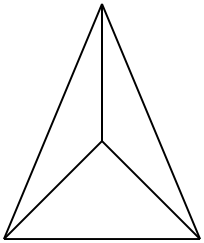
\includegraphics[height=1.3in]{../images/graphs/k4.png}
			\label{fig:images_graphs_k4}
		}\hspace{1.5em}
		&
		\subfigure[$K_5$.]{
			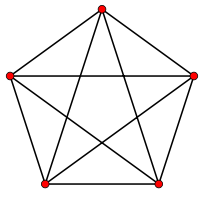
\includegraphics[height=1.3in]{../images/graphs/k5.png}
			\label{fig:images_graphs_k5}
		}		
	\end{tabular}
	\caption
	[$K_4$ and $K_5$.]
	{Examples of a planar and a non-planar graph; the complete graph
	with 4 and 5 nodes, respectively.}
\end{figure}

There exist different methods for planarization. Cai et al. present an
$O(m\log n)$-time algorithm for finding the \emph{maximal planar subgraph}
\cite{Cai1993}. One can also try to find the drawing with the minimum number
of edge crossings. This problem is NP-hard as shown in \cite{Garey1983}, but
heuristics for minimizing the number of crossings are given in
\cite{Ferrari1969}. Another planarization technique is called
\emph{splitting}. A splitting operation converts a node $v$ to two nodes $v_1$
and $v_2$, attaching the neightbours of $v$ to either $v_1$ or $v_2$.
Heuristics for planarization by splitting are discussed in \cite{Eades1993}. 

\section{Planar Representations}

A \emph{planar representation} is a data structure that represents possible
planar embeddings of graph, i.e. which combinations of node positions give
rise to a planar graph. Many drawing algorithms construct a drawing from a
planar representation -- first by testing for planarity, then contructing a
planar representation and then use a drawing algorithm to draw this
representation.

A \emph{path addition} approach to planarity testing was presented by Hopcroft
\cite{Hopcroft1974,Deo1976}. Another approach called the \emph{vertex
addition} approach is presented in \cite{Booth1976}. Both of these methods for
planarity testing run in linear time. Chiba et al. modified the methods of
\cite{Booth1976} to construct planar representations \cite{Chiba1985}.

\section{Straight-line Drawing}

For an undirected graph, the graphic standard with all edges represented by
straight lines is called a \emph{straight-line drawing}. Eades presented an
approach to straight-line drawing using a spring-metaphor
\cite{Eades1984,Fruchterman1991}. In this system, vertices are regarded as
rings and edges are regarded as springs. The springs attract the rings if they
are too far apart and repel them if they are too close. This category of
drawing algorithms is called ``force-directed'' algorithms.

In \cite{Lipton1985} the authors present an approach that focus mainly on
capturing symmetries in the graphs. However, this approach is computationally
very expensive when compared to \cite{Eades1984}.

Another approach is to associate an energy function to a drawing, representing
the ``quality'' of the drawing with respect to the chosen aesthetic measures
by an amount of energy, and then use simulated annealing to compute the
two-dimensional graph embedding \cite{Davidson1996}.

A mixture of different techniques is presented by Tunkelang in
\cite{Tunkelang1992} that focus on computing the aesthetic cost of a drawing,
the order of node placement and local optimization techniques.

It was shown early that every planar graph can be drawn as a planar
straight-line drawing \cite{Wagner1936,Fary1948,Stein1951}. Tutte studied
\emph{convex drawings} of planar graphs, which is a drawing where the faces
consisting of the graph edges are all convex polygons \cite{Tutte1960} (Figure
\ref{fig:images_graphs_convex_1}). Thomassen furthermore characterized the
class of graphs that can be embedded in a convex drawing \cite{Thomassen1980},
and Chiba et al. give a linear time algorithm for making convex drawings using
Thomassen's results \cite{Chiba1984}.
\begin{figure}[htp]
	\centering
		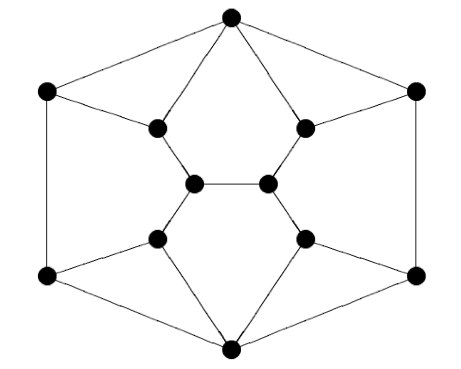
\includegraphics[height=1.5in]{../images/graphs/convex_1.png}
	\caption
	[A convex drawing of a graph.]
	{A convex drawing of a graph. All faces are drawn as convex 
	polygons. (Taken from \cite{DiBattista1994}, Figure 8.)}
	\label{fig:images_graphs_convex_1}
\end{figure}

An aesthetic measure for straight-line drawings is the total edge length.
Becker et al. show that the there is a unique and convex optimal straight-line
drawing with the external face a prescribed convex polygon \cite{Becker1987}.
On the other hand, constructing a planar straight-line drawing with a
prescribed edge length, as measured by the Euclidean metric, is NP-hard
\cite{Eades1990}. 

The performance of several drawing algorthms are compared in \cite{Jones1991}.
The quality of the drawings is measured in terms of the standard deviation of
angle size between edges, the edge length and the face area.

\section{Orthogonal Grid Drawing}

The graphic standard where all edges are either parallel or orthogonal and
fixed to a grid is called \emph{orthogonal grid drawing}, see Figure
\ref{fig:images_graphs_orthogonal_1}. This type of drawing was originally
motivated by circuit layout problems. A common aesthetic measure for this type
of graph is the amount of bends on edges, as well as the area that the drawing
covers. These aesthetics not only affect readability; in circuit design they
have a direct impact on the quality of the circuit that is produced.

In \cite{Batini1984,Tamassia1988} the authors present a general method for the
construction of orthogonal grid drawings. It can be subdivided into three
steps: first the graph is planarized, then an orthogonal shape is computed
based on the planarized graph, and finally this shape is made as compact as
possible to produce the final drawing. This general approch allows orthogonal
grid drawings of many different types of graphs.

It is an NP-complete problem to determine whether a graph can be embedded in a
planar orthogonal drawing without bends, whence the bend-minimization problem
is NP-hard \cite{Garg1994}.

\begin{figure}[htp]
	\centering
		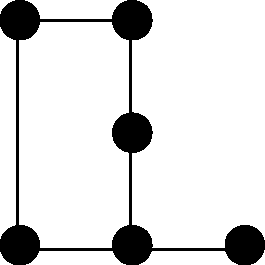
\includegraphics[height=1in]{../images/graphs/orthogonal_1.pdf}
	\caption{An orthogonal grid drawing of a graph.}
	\label{fig:images_graphs_orthogonal_1}
\end{figure}

\section{Visibility Representations}

In a \emph{visibility representation}, each vertex is represented as a
horizontal line and each edge as a vertical line. The vertical lines intersect
exactly those horizontal lines that the corresponding edges connect
\cite{Duchet1983}, see Figure \ref{fig:images_graphs_visibility_repr_1}.
Visibility representations were originally motivated by VLSI layout because it
gives regular, modular graphs \cite{Schlag1985}.

An overview of different classes of visibility representations and linear time
drawing algorithms is given by Tamassia et al. \cite{Tamassia1986}. Often the
first step in creating a visibility representation of an undirected graph is
to create a \emph{bipolar orientation} of it. A bipolar orientation of an
undirected graph is an orientation of the edges of the graph such that the
resulting \emph{directed} graph is acyclic and has excatly one source -- a
vertex having only outgoing edges -- and exactly one sink -- a vertex with
only incoming edges. Properties of bipolar orientations are investigated in
\cite{Fraysseix1993}.

\begin{figure}[htp]
	\centering
	\subfigure{
		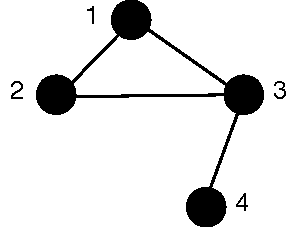
\includegraphics[height=1in]{../images/graphs/visibility_repr_1.pdf}
	}
	\subfigure{
		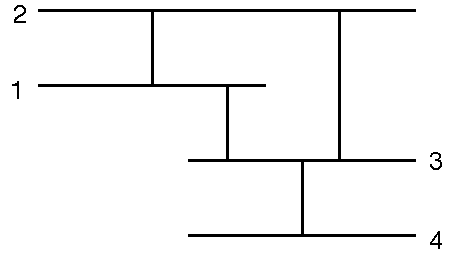
\includegraphics[height=1in]{../images/graphs/visibility_repr_2.pdf}
	}
	\caption{A graph $G$ and its visibility representation.}
	\label{fig:images_graphs_visibility_repr_1}
\end{figure}


\section{Miscellaneous Graphic Standards}

Ozawa proposes a graphic standard where all vertices are dots on a straight
line, and edges are drawn as half-circles over or under the line
\cite{Ozawa1980}, as exemplified in Figure \ref{fig:images_graphs_circles_1}.
\begin{figure}[htp]
	\centering
		
\includegraphics[height=0.6in]{../images/graphs/circles_1.pdf}
	\caption
	[The approach suggested by Ozawa.]
	{The approach suggested by Ozawa \cite{Ozawa1980}.}
	\label{fig:images_graphs_circles_1}
\end{figure}

For cubic graphs that are planar, Kant proposes a method for placing them on a
hexagonal grid in linear time \cite{Kant1992}.

Problems in architectural design motivated a graphic standard where vertices
are represented by polygons and an edge between two vertices are represented
as the two corresponding polygons being geometrically adjacent
\cite{Bhasker1988}. A variant of this graphic standard is the
\emph{tessellation representation} in which vertices, edges and faces of a
planar embedding of a graph is represented as rectangles, and adjacencies
between rectangles correspond to incidencies in the graph \cite{Tamassia1989}
-- see Figure \ref{fig:images_graphs_tessellation}.

\begin{figure}[htp]
	\centering
	\subfigure{
		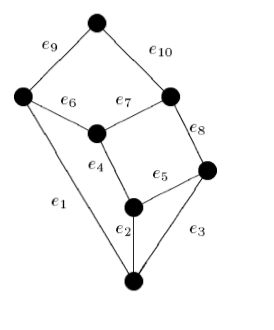
\includegraphics[height=2in]{../images/graphs/tessellation_1.png}
	}
	\subfigure{
		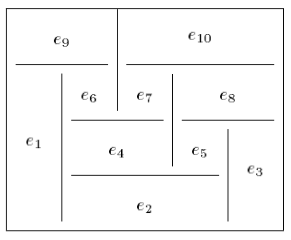
\includegraphics[height=2in]{../images/graphs/tessellation_2.png}
	}
	\caption
	[A tessellation representation of a graph.]
	{A tessellation representation of a graph. (Taken from \cite{DiBattista1994}, Figure 11.)}
	\label{fig:images_graphs_tessellation}
\end{figure}

Dickerson et al. present the graphic standard \emph{confluent drawing} along
with heuristics for it \cite{Dickerson2005} -- see Figure
\ref{fig:images_graphs_confluent}. In this approach, groups of edges are
merged together to what the authors call ``tracks'', and the graph can then be
drawn without crossing edges.

\begin{figure}[htp]
	\centering
	\subfigure{
		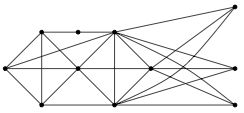
\includegraphics[height=1in]{../images/graphs/confluent_1.png}
	}
	\subfigure{
		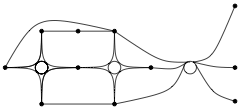
\includegraphics[height=1in]{../images/graphs/confluent_2.png}
	}
	\caption
	[A non-confluent and a confluent drawing of the same graph.]
	{A non-confluent and a confluent drawing of the same graph. 
	(Taken from \cite{Dickerson2005}, Figure 5.)}
	\label{fig:images_graphs_confluent}
\end{figure}

\section{Directed Graphs}

Directed acyclic graphs are used to represent hierachical structure, for
instance in dependency graphs. It is desirable to draw these graphs such that
all edges point in the same direction. A drawing is called \emph{upward} if
all edges are pointing upwards. 

For directed graphs there exists the notion of \emph{upward planarity}, which
corresponds to the notion of planarity for undirected graphs. A graph is
upward planar if it can be drawn without any crossing edges and with all edges
pointing upwards. Algorithms for drawing upward planar graphs are given in
\cite{DiBattista1988}. 

A drawing that is upward planar and in which all edges are straight lines is
called a \emph{Hasse diagram}. These drawings are commonly used to represent
partially ordered sets, and a drawing algorithm is given in
\cite{Jurgensen1983}. Thomassen characterizes the graphs that have a Hasse
diagram in \cite{Thomassen1989}. 

When drawing a directed acyclic graph, three steps corresponding to the case
with an undirected graph are used: the graph is upwards planarized, a planar
representation is found and this representation is drawn with a drawing
algorithm. It is an NP-complete problem to test whether a graph is upward
planar in general \cite{Garg1994}, but polynomial time algorithms exist for
special cases, among others in \cite{DiBattista1990}. A survey of efficient
algorithms that take a planar representation and draw the graph is given in
\cite{Tamassia1990}.

If all vertices are placed on a set of straight, equally spaced lines, with
edges going only between vertices on different lines and not overlapping, the
drawing is said to be a \emph{hierachical drawing}. The procedure for making a
hierachical drawing has three steps: assign vertices to the different lines
such that all edges point upwards, find a permutation of the vertices in which
no edges overlap and finally tune the positions of the vertices to minimize
the number of edge bends. A comprehensive approach is presented by Sugiyama
et al. \cite{Sugiyama1981}. The algorithms used at the three steps are
analysed in \cite{Lin1992}.

For a directed graph that contains cycles it is often desirable to represent
the \emph{flow} of the graph. This is done by maximising the number of edges
that point upwards, which is equivalent to finding the minimum number of edges
that need to be reversed in order to make the graph acyclic. This problem is
in general NP-complete, but there exist polynomial time algorithms for special
cases \cite{Frank1981}. Heuristics for the problem are discussed in
\cite{Berger1990}. After making a graph acyclic, the techniques previously
mentioned can be used. If the representation of flow in the graph is not
important, the acyclic techniques can be applied directly, ignoring the edge
directions.

\section{Issues Related to Large Graphs}

When the size of the graph to be drawn becomes sufficiently large, a host of
new issues appears. First of all there is the question about performance;
several algorithms discussed above and in the referenced papers would be
unacceptably slow if applied to a graph with e.g. $10^4$ nodes and
$3\cdot10^4$ edges. It can therefore sometimes be necessary to alter the
methods. Furthermore there is the problem of room -- there simply has to be
enough room on the monitor for the drawing to fit. In this section we will
briefly discuss a few such methods. A more rigorous study can be found in
\cite{Herman2000}.

For a large graph with $10^4$ nodes and $3\cdot10^4$ edges, the probability
that the graph is planar is very small, and since a planarity check on such a
graph will be slow it is usually just skipped. 


Since a lot of applications of graph drawing techniques operate with large
graphs that cannot be placed all at once on a normal computer monitor, methods
to single out special parts of the drawing and only show these have been
developed. Since one will usually be interested in the whole graph, or at
least most of it, navigational methods have also been studied. 

One method to solve the problem of showing a huge drawing on a relatively
small monitor is to use a ``fisheye'' effect. This effect functions as a
``magnifying glass'' that highlights, or enlarges, the area of the graph
currently in focus while at the same time minimizing the other parts. Using
this, a user can navigate and study a large graph that would otherwise be
drawn with node and edge representations too small for the human eye to
discern. The method utilizes a distortion function, $d:[0,1]\mapsto[0,1]$,
that monotonically maps the interval $[0,1]$ to itself. Figure
\ref{fig:images_fisheye_distortion} shows an example of two distortion functions
as well as an illustration of the effects on a plane.
\begin{figure}[htp]
	\centering
	\subfigure{
		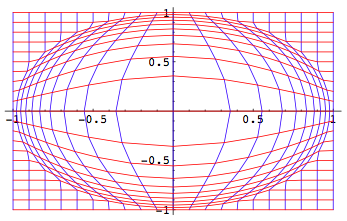
\includegraphics[height=1.7in]{../images/fisheye_distortion.png}
	}
	\subfigure{
		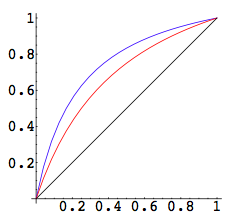
\includegraphics[height=1.9in]{../images/fisheye_distortion_func.png}
	}
	\caption
	[Distortion of a regular grid and a distortion function.]
	{Distortion of a regular grid along with an example of a distortion function. The blue and
	red line represent two different distortion functions, and the black line is 
	the ``normal'', non-distorted view. 
	(Taken from \cite{Herman2000}, Figure 17 and 18.)}
	\label{fig:images_fisheye_distortion}
\end{figure}

A related method is to draw the graph in a hyperbolic coordinate system
instead of an Euclidean. This gives the impression that the graph is drawn on
a sphere, where the graph elements lying on the part of the sphere pointing
towards the observer appear to be enlarged. If this sphere can be rotated by
the user, she can decide which parts of the graph to enlarge and which not,
analogously to the fisheye effect.

If a graph drawing algorithm can reduce the amount of elements, large-scale
structures can be represented in a comprehensible fashion, even though the
underlying graph may contain too many nodes for a normal drawing method. This
approach is called \emph{clustering}. The essence of the method is to find
groups, or clusters, in the graph that have something in common and then draw
the graph consisting of the clusters instead of the original graph. If the
clustering algorithm is chosen properly, structures in graphs otherwise
seemingly chaotic can be easily discerned. One challenging part of the
approach is to find a sensible balance between number of clusters and number
of nodes per cluster, as well as devising a fitting similarity measure for the
clustering algorithm. 

% Relatedly, methods that can intelligently hide parts of the graph deemed
% non-interesting can also greatly increase the clarity of the drawing. 

% clustering
% hiding
% no planarity check/solution
% incremental exploration
% focus+context (hyperbolic, fisheye etc.)
% navigation



% G. Di Battista, P. Eades, R. Tamassia, and I. G. Tollis, 
%   Graph Drawing, Prentice Hall, Upper Saddle River, NJ, 1999.

% Pilehoveder?

